\chapter{Financement et rôle de la monnaie}
\section{Définitions}
\subsection{Les caractéristiques de la monnaie}
\textcolor{BrickRed}{La monnaie est un actif financier} : c'est une créance pour les agents qui la détiennent, c'est une dette pour les agents qui l'émettent \newline
\textcolor{BrickRed}{La monnaie est la liquidité par excellence} : elle est négociable contre tout bien, service ou créance. Permet de s'acquitter de toute dettes rapidement \newline
\textcolor{BrickRed}{La monnaie est un actif financier non rémunéré (en général) qui n'est pas nécessairement remboursé} \newline

\subsection{Les fonctions de la monnaie}
\textcolor{BrickRed}{La monnaie est une mesure des valeurs} \newline
\textcolor{BrickRed}{La monnaie est un intermédiaire des échanges} \newline
\textcolor{BrickRed}{La monnaie est un instrument de réserve} : elle permet d'épargner en vue de consommations futures
\newpage
\section{Les écoles de pensée}
\subsection{Remarques}
\textcolor{BrickRed}{Stock nominal et stocl réel de monnaie}
\begin{center}
    \Large{\fbox{$\Delta S_{R} = \frac{\Delta S_{N}}{PIB}$}}
\end{center}
\textcolor{BrickRed}{Déflation $\implies$ Stock réel $\nearrow$} \newline
\textcolor{BrickRed}{Inflation $\implies$ Stock réel $\searrow$} \newline
\textcolor{BrickRed}{Le pouvoir d'achat de la monnaie dépend de la quantité de biens et de services qu'une quantité de monnaie peut acheter.}
\textcolor{BrickRed}{La demande de monnaie s'analyse comme une demande de pouvoir d'achat.}
\subsection{Théorie quantitative de la monnaie}
\textcolor{BrickRed}{La demande de monnaie s'explique par la quantité de monnaie nécessaire pour faire face aux transactions} \newline
\begin{center}
    \Large{\fbox{$MV = PT$}}
\end{center}
Avec :
\begin{itemize}
    \item $M$ : quantité de monnaie demandée
    \item $P$ : le niveau général des prix
    \item $T = aY$ : l'activité économique (transactions)
    \item $V$ : vitesse de circulation de la monnaie
\end{itemize}
équation de Cambridge :
\begin{center}
    \Large{\fbox{$\frac{M}{P} = kY$}}
\end{center}
$k = \frac{a}{V}$
\newpage
\begin{itemize}
    \item Encaisse réelle de de transaction et de précautions $M_{t}$
\begin{center}
    \Large{\fbox{$m_{t}=L_{1}=\frac{Y}{V}$}}
\end{center}
    \item Encaisse de spéculation $M_{s}$
\begin{center}
    \Large{\fbox{$m_{s}=L_{2}(i)$}}\footnote{Fonction $\searrow$ du taux d'intérêt}
\end{center}
\end{itemize}
\subsection{Friedman et la vision monétariste}
Vision opposée à Keynes (revenu courant). Les monétaristes rejoignent la \textbf{théorie quantitative (néoclassqiue)} en ce qui concerne les agents face à un \textbf{accroissement de la quantité de monnaie} en circulation : \textbf{les agents ajustent les achats en consommant, ce qui fait augmenter les prix}
\subsubsection{Théorie du revenu permanent}
C'est la somme des revenus attendus du patrimoine humain et du patrimoine matériel sur toute la durée de vie de l'agent.
\begin{center}
    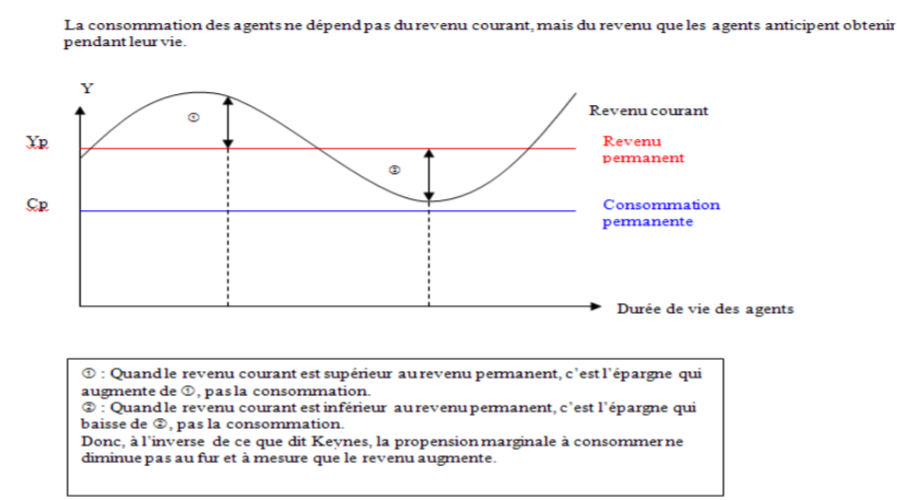
\includegraphics[scale=0.5]{Pics/Theorie_revenu_permanent.png}
\end{center}
\section{La création monétaire}
\subsection{Prêts et font de dépôt}
\begin{center}
    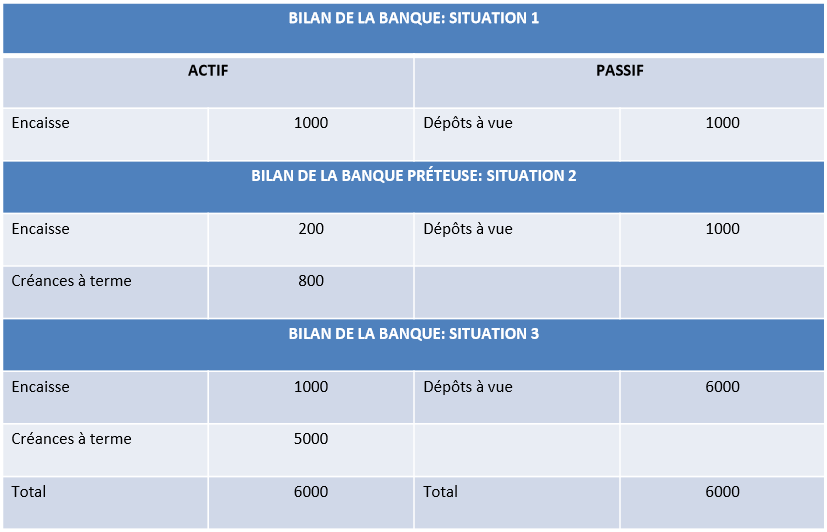
\includegraphics[scale=0.75]{Pics/Pret_et_fond_de_depot.png}
\end{center}
\subsection{Couverture}
\textcolor{BrickRed}{Couverture} : Part de l'actif bilan conservée en créance liquide dans les banques centrales (billets, or...) \newline
\textcolor{BrickRed}{Taux de couverture} : 
\begin{center}
    \Large{\fbox{$T = \frac{C}{E}$}}
\end{center}
\begin{itemize}
    \item $T$ : taux de couverture
    \item $C$ : créances sur la banque centrale
    \item $E$ : Engagemen à vue, dépôts 
\end{itemize}
\subsection{Multiplicateur de dépôts}
Multiplicateur de crédit :
\begin{center}
    \Large{\fbox{$M = \frac{m}{1-c} = \frac{m}{r} = mk$}}
\end{center}
\subsection{Banque centrale}

\begin{itemize}
    \item \textcolor{BrickRed}{La monnaie centrale} : monnaie émise par la banque centrale (monnaie fiducaire : billets)
    \item \textcolor{BrickRed}{La monnaie créée par le crédit bancaire}
    \begin{center}
        \Large{\fbox{$M = \frac{B}{r} = Bk$}}
    \end{center}
\end{itemize}
\begin{itemize}
    \item $M$ : monnaie créée
    \item $B$ : monnaie centrale
    \item $r$ : taux de réserve \footnote{Taux de réserves liquides obligatoires qui impose au système bancaire de constituer une certaine proportion de ses dépôts sous forme de monnaie centrale}
    \item $k$ : multiplicateur tq $k > 1$
\end{itemize}
\newpage
\subsection{Liquidité bancaire}
\begin{itemize}
    \item \textcolor{BrickRed}{Liquidité bancaire} : disponibilité des banques en monnaie centrale
    \item \textcolor{BrickRed}{opérations en monnaie centrale} : opérations interbancaires et facteurs autonomes de liquidité \footnote{Liquidité échangées entre banques mais aussi entre zones de liquidité. Ex : un agent consomme aux USA $\implies$ la banque centrale Américaine achète de la liquidité auprès du consommateur en zone euro}
    \item \textcolor{BrickRed}{Refinancement par la banque centrale (IMPORTANT)} : la banque centrale prête aux banques des disponibilités de monnaie centrale
    \item \textcolor{BrickRed}{Les besoins en monnaie centrale fournissent à la banque centrale le smoyens de réguler la création des liquidités par le jeu des opérations de refinancement des banques}
\end{itemize}
\subsection{Les instruments de la politque monétaire de l'eurosystème}
\begin{itemize}
    \item \textcolor{BrickRed}{Les opérations d'open market} : pilotent le taux d'intérêt et de liquidité bancaire
    \item \textcolor{BrickRed}{Les facilités permanentes} : 
    \begin{itemize}
        \item \textcolor{BrickRed}{Facilités de prêt marginal} : permet d'obtenir des liquidités au jour le jour
        \item \textcolor{BrickRed}{Facilité de dépôt} : permet d'effectuer des dépôts au jour le jour
    \end{itemize}
    \item \textcolor{BrickRed}{Les réserves obligatoires} : stabilisent le taux d'intérêt du marché monétaire et permet de créer le besoin structurel de refinancement.
\end{itemize}
\newpage
\subsection{Le financement de l'économie}
\begin{center}
    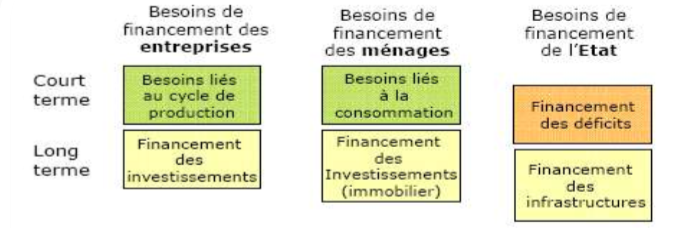
\includegraphics[scale=0.8]{Pics/Financement_economie.png}
\end{center}
Les banques centrales sont mandatées par les états pour réguler le monopole monétaire sur chaque continents. Les autres banques dites \textbf{banques secondaire} ou de \textbf{second rang} s'endettent de la monnaie centrale en la distribuant aux consommateurs. C'est un \textbf{crédit bancaire}.
\subsection{Formes de financement}
\begin{itemize}
    \item \textcolor{BrickRed}{Economie d'endettement} : création monétaire avec les banques de second rang et banques centrales ("usine de monnaie") \newline
    Le financement passe obligatoirement par les banques : c'est \textcolor{BrickRed}{l'intermédiation bancaire}
    \item \textcolor{BrickRed}{Economie des marchés financiers} : agents qui dégagent des capacités de financement directement sur les marchés financiers.\newline
    C'est \textcolor{BrickRed}{la désintermédiation}
\end{itemize}
\newpage
\section{Histoire des faits économiques}
Après la seconde guerre mondiale, le financement par crédit est la seule solution envisageable (pas d'épargne ches les agents privés). L'état réorganise le système bancaire : il est omniprésent. \newline
C'est un système qui augmente la masse monétaire et donc \textbf{inflationniste}. En 1973, avec le premier choc pétrolier, l'inflation est très forte et pousse les agents à s'endetter $\implies$ \textbf{surendettement}
\newline
Pendant les 30 glorieuses (1953-1970) : politique d'inspiration keynésienne, \textbf{Stop and Go}. \newline
A partir de 1973 : détérioration rapide des soldes budjétaires. \newline
Années 1980 : lutte contre l'inflation. \newline
\textbf{Pour lutter contre l'inflation, il faut hausser le taux dintérêt pour réduire le nombre de crédits}. Pour avoir un financement, il faut se procurer les ressources sur les \textbf{marchés capitaux}
\newpage
\subsection{Marchés capitaux}
\begin{itemize}
    \item \textcolor{BrickRed}{Marché monétaire} : échange des sur capitaux à court terme \footnote{$<$ 7 ans}
    \item \textcolor{BrickRed}{Marché financier} : offre et demande sur le long terme \footnote{$>$ 7 ans}
    \item \textcolor{BrickRed}{Les actions} : Les détenteurs d'actions sont propriétaires d'une partie de l'entreprise qui veulent se financer. Le revenu des actions dépend du profit des entreprises. une partie des profits est reversé sous forme de dividendes aux actionnaires.
    \item \textcolor{BrickRed}{Les obligations} : dettes avec un taux
\end{itemize}